\documentclass[12pt]{article}

% Language setting
% Replace `english' with e.g. `pathspanish' to change the document language
\usepackage[english]{babel}

% Set page size and margins
% Replace `letterpaper' with`a4paper' for UK/EU standard size
\usepackage[a4paper,top=2cm,bottom=2cm,left=3cm,right=3cm,marginparwidth=1.75cm]{geometry}

% Useful packages
\usepackage{amsmath}
\usepackage{graphicx}
\usepackage{subfig}
\usepackage[colorlinks=true, allcolors=black]{hyperref}

\begin{document}

%title
\title{\underline{Project report - AutoPylot}}
\date{March 2022}


\author{%
    \\
    Alexandre Girold\\
    Mickael Bobovitch \\
    Maxime Ellerbach \\
    Maxime Gay \\ \\
    Group: Autonomobile 
    }

\maketitle

\centerline{
\includegraphics[height=8cm]{../../logos/logo-transparent-black.png}}
\newpage

\tableofcontents
\newpage

\section{Introduction}

\subsection{Project presentation}
Autonomous vehicles and more specifically self-driving cars have grasp the attention of many people for good or ill. In this spirit, we have decided with the Autonomobile team to create our first ever project, AutoPylot. The name of our team is of course full of meaning in that regard. Autonomobile is a two-word name, the first one a French word for autonomous : "Autonome", the second one a French word for car : "Automobile". These two-word combined literally mean Autonomous car.\\

What is AutoPylot's goal ? 
Drive itself on a track and win races. It may, at first glance seem very simple but not everything is at it seems. Yet we will try to make it as easy to understand as possible, without omitting crucial information. To achieve our goal, we need to solve many other problems. Those problems can be separate into two distinct groups. \\

The first one would be the software part. Indeed, in this project we will need to learn and acquire certain skills, from teamwork to coding in different languages. With those newly acquired skills we will be able to bring machine learning to our car to make it drive itself. This leads use directly to our second part, the more tangible one : hardware. Indeed, as we will progress in our work, we will need to see the results of our work in real life condition. This means implementing our code to a functioning car which will be able to race on a track. \\

This project will lead by a team of four young developers, Maxime Ellerbach, Mickael Bobovitch, Maxime Gay and Alexandre Girold. In this project work will be divided equally amongst all of us, sometimes we will have to work together to achieve our very tight time frame. 

\subsection{Team members}

% Write a small paragraph about yourself, what you like, what you did in the past. Everything is valuable !
\subsubsection{Maxime Ellerbach}
I am a curious and learning hungry person, always happy to learn and collaborate with new people ! Programming, robotics and tinkering has always attracted me. Writing code and then seeing the results in real life is something that I find amazing ! I had multiple projects in this field : Lego Mindstorms, a robotic arm, more recently an autonomous car and even a simulator in unity to train even without a circuit at home ! Even if I know quite well the domain of autonomous cars, there is always something new to learn. I look forward working with this team full of hard-working people on such a fun project !

\subsubsection{Mickael Bobovitch}
Roses are red. Violets are blue. Unexpected “Mickael BOBOVITCH“ on line 32. Hello I am a French Student with Russian parents. Lived half of my life in Moscow. Passionate in web dev, servers, and business. Started programming at 13 years old. Created many projects. I like to learn everything, from AI, to UI, from Hardware to Software. Actually I am like OCaml, you need to know me well to appreciate me.

\subsubsection{Maxime Gay}
I am 18 years old,  and I am crazy about investment, finance and especially cryptocurrencies and blockchain. I already worked with a team on different Investment projects and during summer Jobs, but this is the first time that I am working on such a  project. Furthermore, I am a beginner in computer Science and autonomous car. However, I am impatient to learn new skills with this incredible team. 

\subsubsection{Alexandre Girold}
I am already getting old. I am 19 years of age, yet I am full of resources. I am delighted to be able to learn something new. There are many things which I enjoy from programming to geopolitics. I know this project will push me toward a better me and make great friends along the way. 

\subsection{State of the art}
In this section, we will try to see what was previously made in this sector of industry.
It would not be realistic to compare our 1:10 project to real sized cars such as Tesla's, simply because in a racing environment,
we don't need to deal with such an amount of safety: pedestrian detection, emergency braking, speed limit detection and other.
So we will only see miniature autonomous racing framework that we would likely race against.\\

The most known is called "DonkeyCar", created by Will Roscoe and Adam Conway in early of 2017. Most of the models trained with DonkeyCar are behavior cloning models, meaning models that tries to replicate the behavior of a driver. This method uses a big amount of images (input) associated to steering angles and throttle (output), it requires the user to drive the car (collect data) prior to training the model: no examples means no training. The lack of training data often leads to the car leaving the track.\\

One other framework worth looking at is one created by Nvidia called "JetRacer" released in 2019. It uses a different approach from DonkeyCar where the user annotates the images by hand by clicking on where the car should go. The model used is similar to what DonkeyCar uses: a Convolutional Neural Network with one input (the image) and two outputs, one for the steering angle and one for the throttle to apply. \\

Both of those frameworks are written in python and use packages such as Tensorflow and OpenCV, we will also use them in our project.
\newpage



\section{Realized tasks}
% TODO

% Bobovitch
\subsection{Telemetry Server}

In our context, we face different problems that may be hard to solve without physically accessing the device. Our code runs on an Rasberry Pi which make difficult the remote control and the debugging process. \\

Moreover, artificial intelligence is a black box. We don't know what's happening during the execution process. That said, once the program has finished to run, logs become available for observation of past events. However, this approach to debugging is not practical and not efficient enough. To better understand the background processes, we decided to use telemetry. It will allow us to collect valuable data in real time. \\

Since we are dealing with an “intelligent” device, we should fully control it at any time. It would be a disaster if the device does not obey us, as it can create a security treat for the environment. As we know, security is always one of the most important point to keep in mind. In the case where the car is moving at full speed towards a child, how could we stop it? The car can damage people, environment or event itself. \\

We came to the point of building a telemetry server in a form of a web application. We benefits from great portability, awesome development process and a powerful UI. It fills all our requirements. The server makes possible for us to communicate with the car in real-time. We can detect any problems before they happen. We can control the car without any limitations. We can remotely stop and restart. We can remotly update settings. And we can remotly view logs and car updates. \\

Now let's see how we implemented this. As seen previously, we have already set up a logger which records the information continuously. Firstly, we extended the functionalities of the logger while maintaining a modular philosophy. The logger gained the ability to send logs and images through a WiFi network. Next we were confrontend to next chalenge : How to send a decent amount of informations to multiple clients of different type (web-browsers and raspberry pi hardware) in real-time ? We choose to use “Socket.io”. This a an excelent open source cross-platform library. “Socket.io” enable us to create bidirectional and low-latency communication. \\

\newpage

Here is a simple exemple of a communication between a client and a server in javascript. This simple API, simplifies our development process and make data transmition more compliant. \\ \\
\centerline{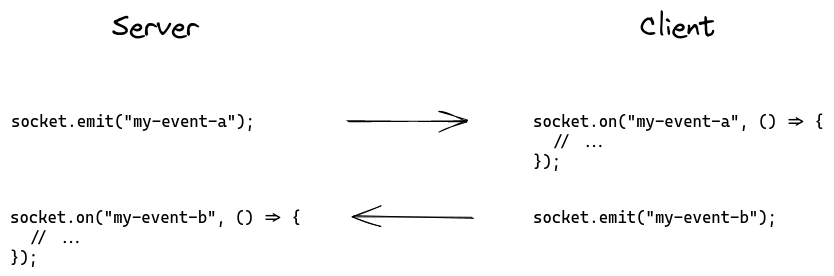
\includegraphics[height=5cm]{../../docs/server-client.png}}

But “Scoket.io” does not stop here. This library is much more powerful. We have the possibility to broadcast a message from the server to all clients : \\ \\
\centerline{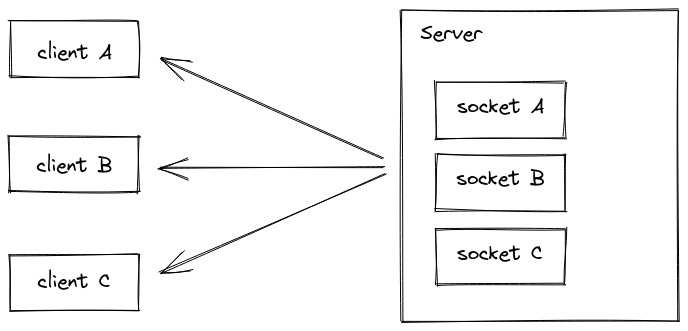
\includegraphics[height=6cm]{../../docs/broadcast-0.png}}

We can even broadcast from a client to other clients: \\ \\
\centerline{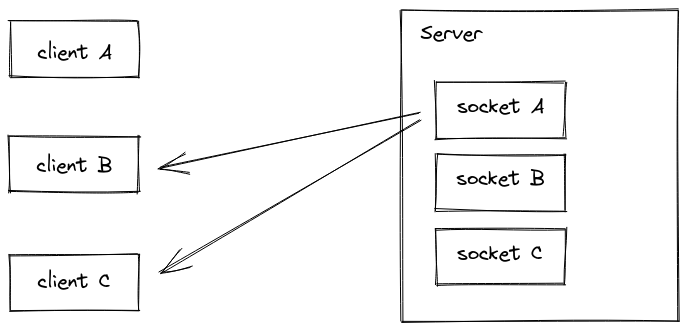
\includegraphics[height=6cm]{../../docs/broadcast-1.png}}

We can even go further by using the concepts of rooms. This means that each client can join a sort of group chart where the server can easily target this group chat: \\ \\
\centerline{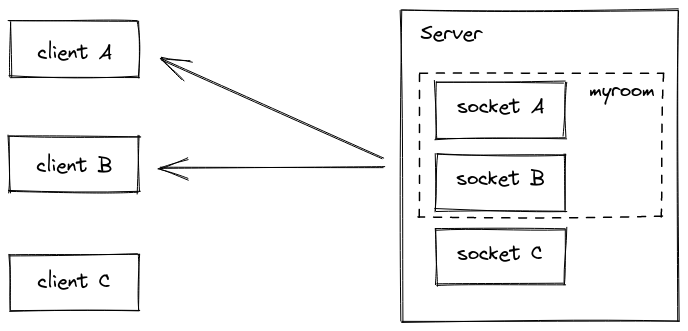
\includegraphics[height=6cm]{../../docs/rooms.png}}

From now, ui-clients|web-clients|people mean a “socket.io” client instance which runs in a web-browser. A car|py-clients is a “socket.io” client instance wich runs on a raspberry pi4. \\

As our main goal is to win races, which implies multiple cars on the track, we have to thinks about a way to manage multiples cars at once. At the same time we wanted every clients of the network would be able to communicate with each other (web-clients with python-clients only). Our design choice was to implement a TV-like mechanism : a web-client can only stream one py-client. And a py-client can send content to an unlimited amount of web-clients, meanwhile a web-clients has the possibility to switch cars at any time. \\

“Socket.io” is just a tool. We developed a high performance server wich is acting as a middleman between clients: \\ \\
\centerline{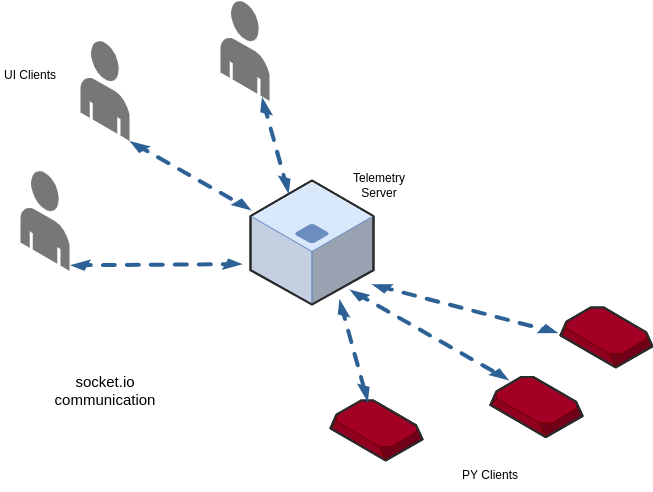
\includegraphics[height=8cm]{../../docs/diagram.png}}

The server uses the JavaScript language (Node JS) as it offers great flexibility, it is very efficient for networking and IO tasks thanks to its language design. Nevertheless, it requires great vigilance because the language is not typed. Any bug could lead to performance issues and memory leaks. But it still remains the best choice for us. We made a great test coverage to extract all bugs. \\

\newpage

The server is battery included, which means it comes with an exeptional UI inspired by the familiar material design by Google. To build the UI we used the “Next.js” framework which is server side rendered react with an API endpoint. “Next.js” is a top-level industry react framework used in many compagnies. We love “Next.js” for it’s simplicity and portability. Here is an exemple of the backend structure which focus on the client side perspective: \\ \\
\centerline{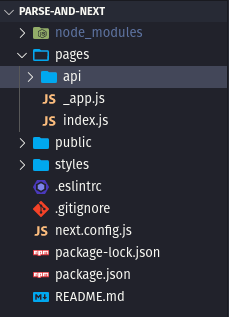
\includegraphics[height=6cm]{../../docs/server-struct.png}}

Here is what we have done : \\ \\
\centerline{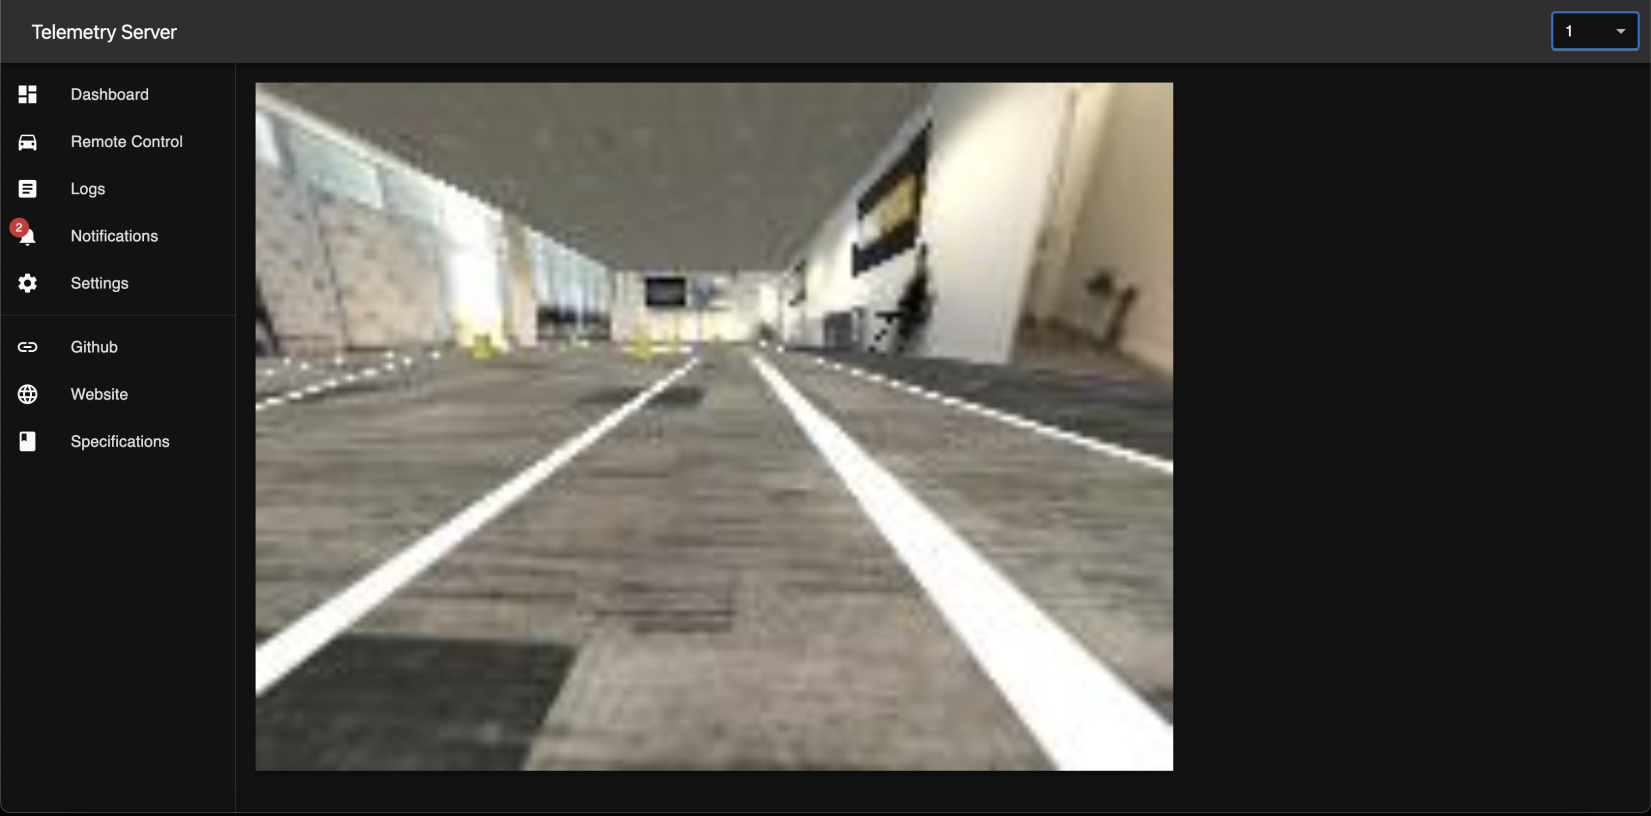
\includegraphics[height=7.5cm]{../../docs/remote-control.png}}
This is the “Remote Control”. This section help us see that the car actualy see in real time. Nothing to say more expted that it’s very cool. We use this in training to we can actualy see better when we drive. \\

\centerline{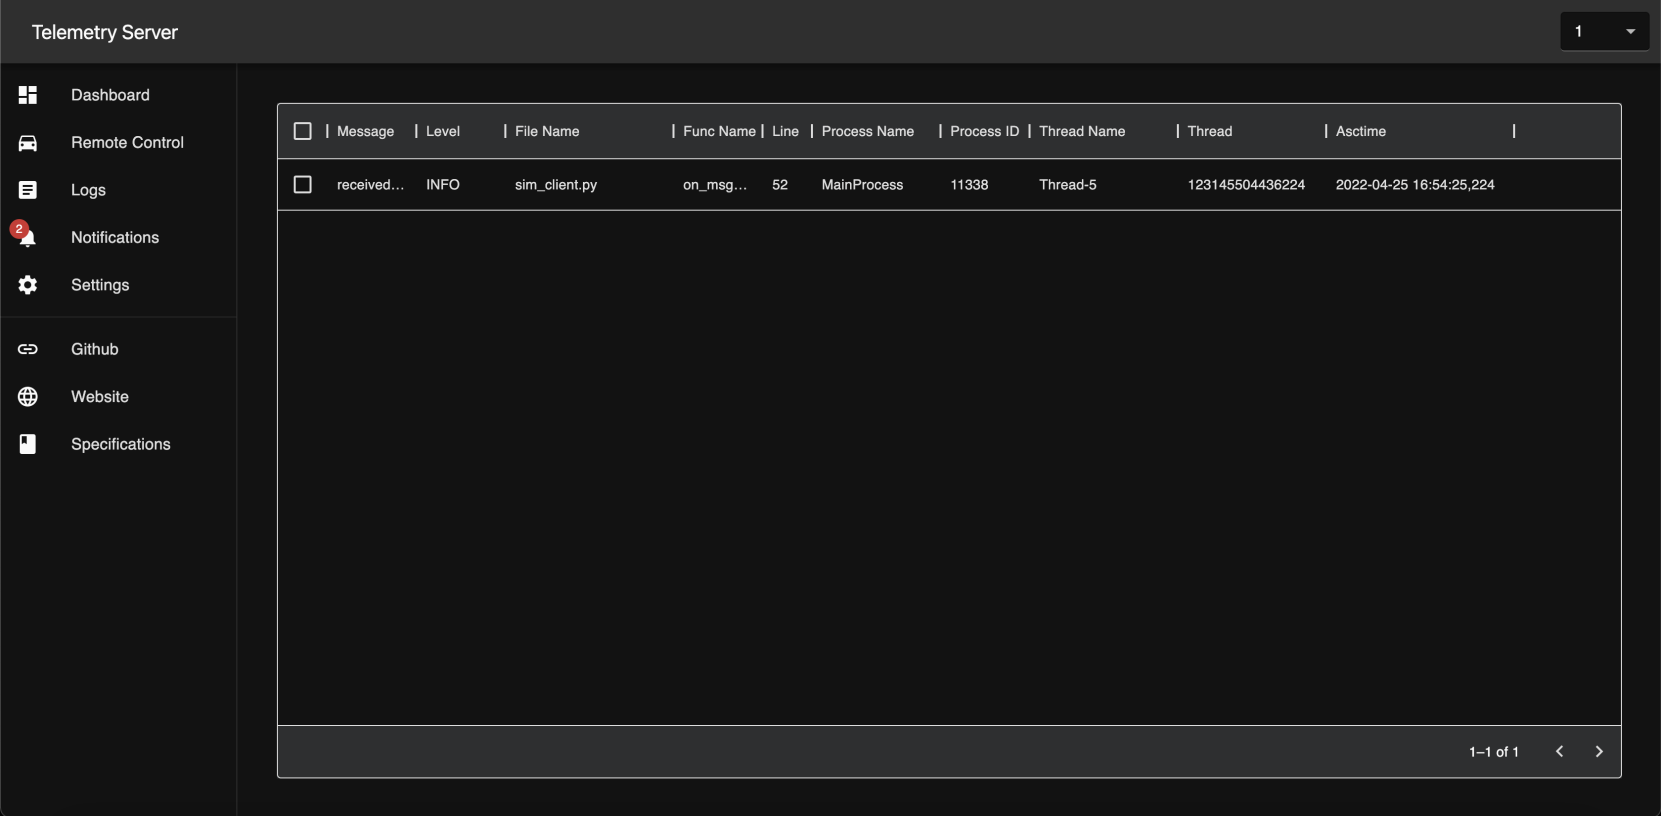
\includegraphics[height=7.5cm]{../../docs/server-logs.png}}
Here are the “Logs”. When someting happen, a new row is inserted. This table support searching. When we have thousands of thousands of logs we can quickly find any message. \\


\centerline{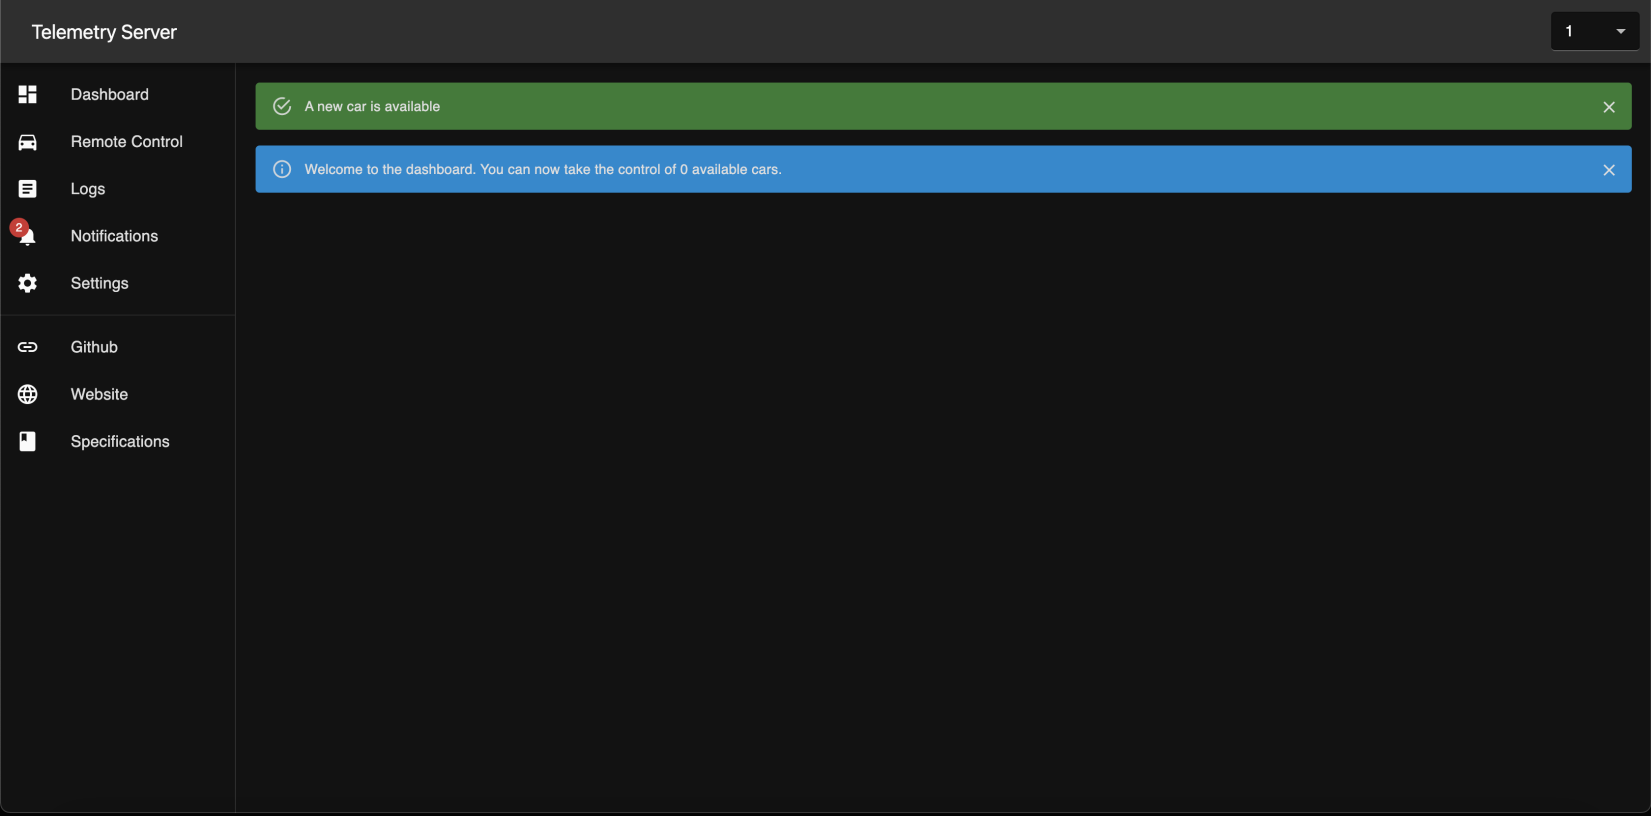
\includegraphics[height=7.5cm]{../../docs/notifications.png}}
Here are the “Notifications”. When something happen, We know it. It might be a new Car available for streaming or maybe the server has an important message to transmit for instance when somebody changed the settings of car.

\centerline{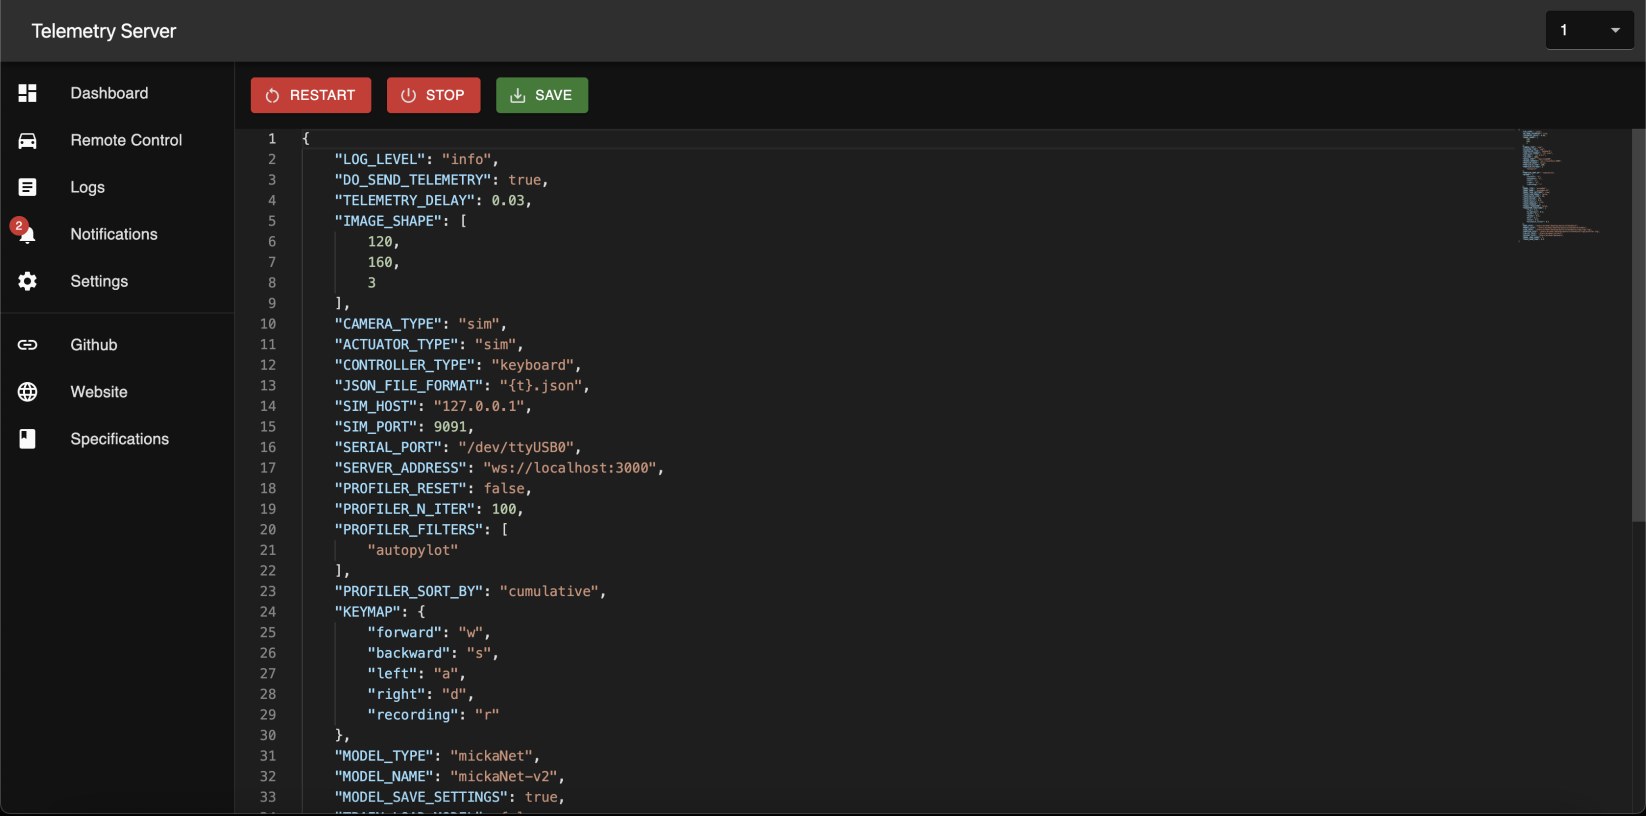
\includegraphics[height=7.5cm]{../../docs/settings.png}}
And eventually here are the “Settings”. This part is crucial. Here we load the “settings.json” from the car. We can update the car’s behaviour, stop or restart with the help of a simple click.\\

In Conclusion this server is the autopylot’s best friend. It’s very easy to use and to install, it can also be accessed on a phone. Every time we use the car, we use this telemetry server. This entire server was developed by hand by our team. We hope to make it even better in the future.

% Ellerbach
\subsection{Some theory}
Before going further into the DeepLearning part, let's have a quick reminder of what is a Neural Network and a bit of theory behind all of that. \\

\subsubsection{Neural Network}
So, what is a Neural Network ? 
A Neural Network or "NN" or "NeuralNet" for short is a black box. The role of a Neural Network is to approximate functions. This can be accomplished with a combination of layers that can be also seen as functions with N parameters and P outputs. Each layer can communicate with the next ones. In most architectures the Neural Network can be visualized as a sequential list of layers, but some are more complex featuring: branches, feedforward and other mystical tricks. \\

This Neural Network by default is only outputting random results, to train it to best approximate our imaginary function, we need one thing: Data ! In our case, we need to predict the next action of our car: steering and throttle from an image: the POV of the car. We can also imagine adding other parameters to our black box like the current speed of the car.
During the training process, the prediction (Forward propagation) the model makes along with the expected value are used to correct the weights and inner parameters of every layer (Backward propagation). To have a well-fitted Neural Network, the more the data we have and the best the quality of that data is, the better ! \\

Neural Networks are mainly composed of fully connected layers (or Dense layers), those are composed of a given amount of neurons. They receive one or more input signals, do calculation on them and then communicates its output signals to the next layer. The output signal is calculated from the sum of every input multiplied by its weight along with the addition of a bias. The output is then going through an activation function before outputting to the next layers. \\

\centerline{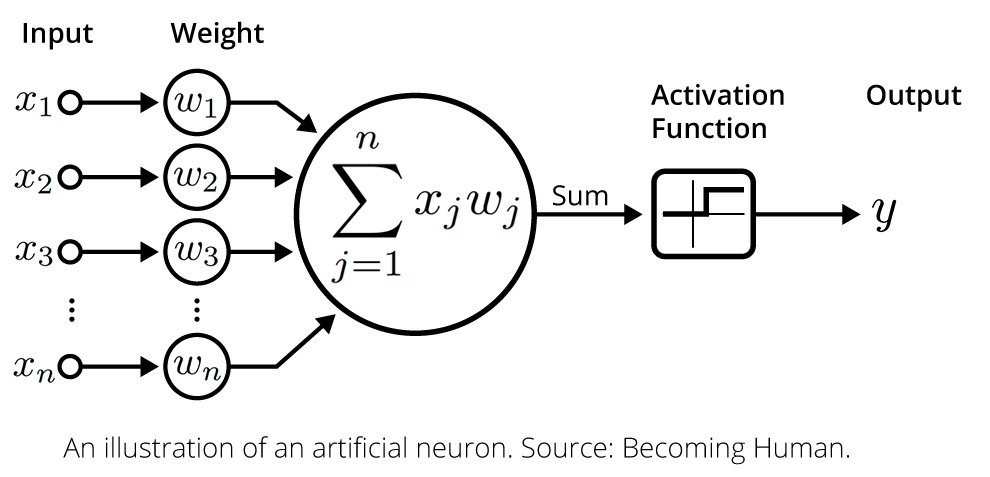
\includegraphics[height=7cm]{../../docs/activation-function.png}}

\subsubsection{Convolutional Neural Network}
So now, what is a Convolutional Neural Network ?
First, a Convolutional Neural Network or "CNN" is a type of Neural Network ! It inherits its name from the kind of layer it has: Convolution layers. \\

What is a Convolution ? 
A convolution is an operation that changes a function into something else. It uses kernels or filters to detect features in a signal. In our case, we use two-dimensional convolution. The signal is the image composed of pixels (usually their values are between 255-0 or 1-0). The main idea behind having convolutions in a Neural Network is to analyze this signal and encode it into a smaller signal. \\
\centerline{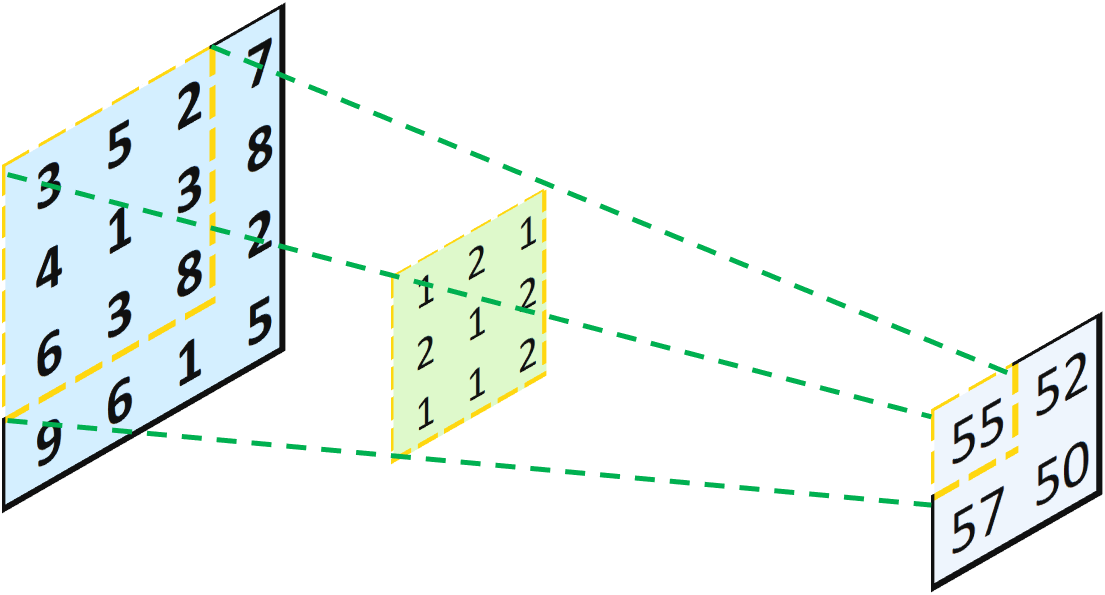
\includegraphics[height=8cm]{../../docs/convolution.png}}

Here you can see the application of a 3x3 convolution kernel on a 4x4 signal, the resulting of the application of this filter is a new signal of size 2x2. The resulting signal is smaller than the input signal, but why is that ? Simply because the kernel here is only applied on the valid areas of the input signal, so the outside border of the signal is lost. To prevent that, we can add zero values around the input filters so that the output size matches the input size. \\
\centerline{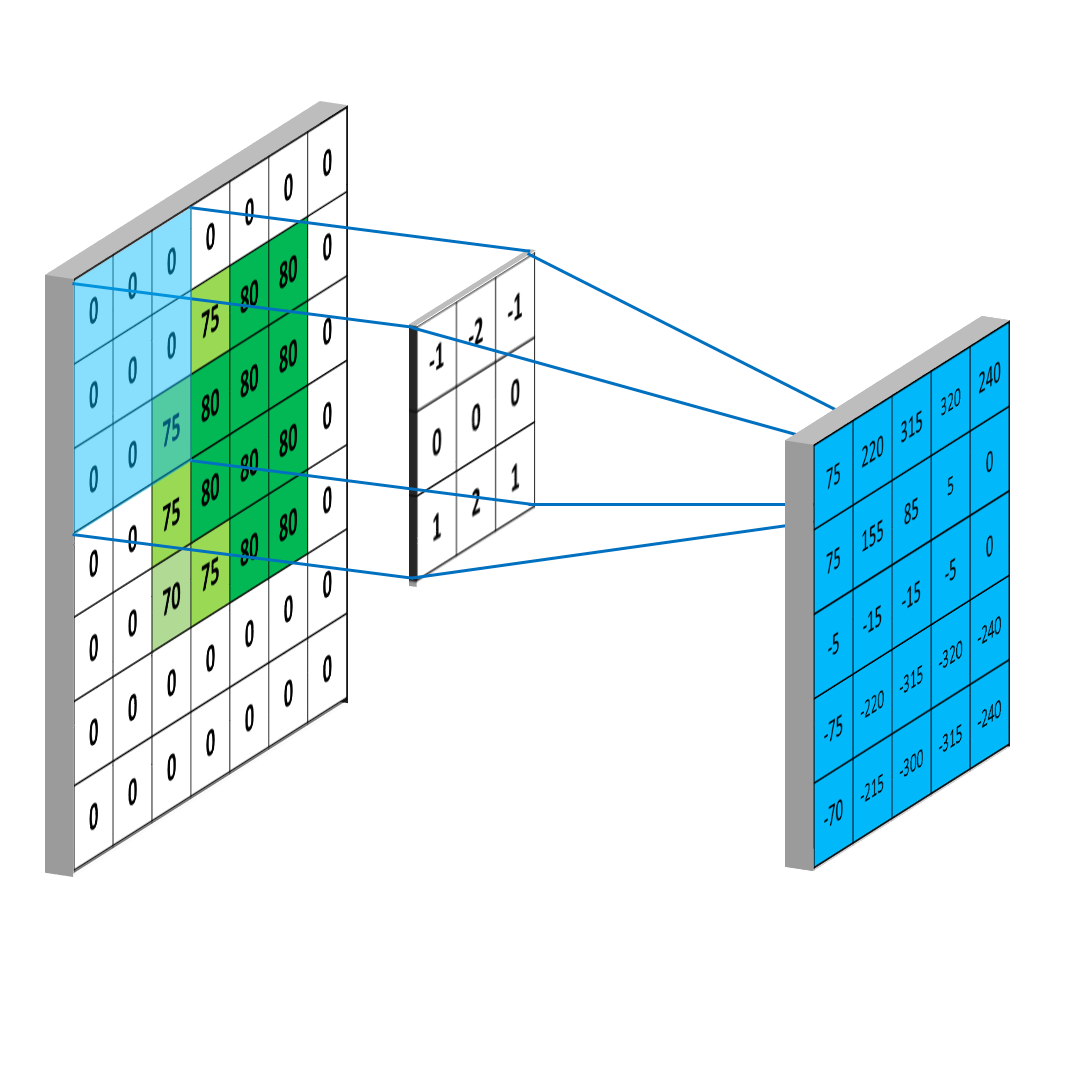
\includegraphics[height=8cm]{../../docs/padding.png}}

Now, as said previously, the main idea of having convolutions is to reduce the size of our image, this can be done by introducing strides to our convolution layers. The amount of movement between applications of the kernel of the input signal is referred as the stride. On the above illustrations, we had a stride of 1 meaning at each step, the kernel moved by 1 pixel. On the illustration below, a 3x3 kernel is applied to a 5x5 signal with strides set to 2 without padding. This results in a 2x2 output signal. \\
\centerline{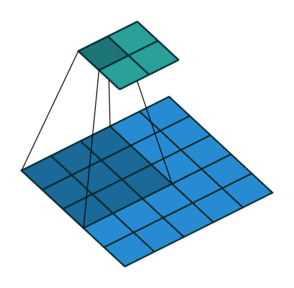
\includegraphics[height=6cm]{../../docs/strides.png}}

Each filter detects simple features from the previous signal but deepest the Convolutional Neural Network is, the more complex the detected features are. Here is an example where we are trying to detect the face of a dog in an image: 
The first convolution layer will detect simple features such as edges on the image, those can correspond to the shape of the dog as well as the shape of other stuff in the image. The second will have in input the already detected edges, from those edges it could detect sets of edges looking like features coming from a dog: ears, eyes, fur. The third one will from those features detect even more complex features and so on.
After the convolutional layers, we are left with something called the latent space of our image. It is the encoded, simplified form of our image where only the key features are left. From those locally detected features, we can then have a look at the big picture by flattening the 2D signals into a 1D vector to be fed into fully connected layers and then answering the question "Is there a dog in the image ?" or "Should we go right or left?". \\

\newpage

\subsubsection{Activation functions}
In some cases, we want our output signal to meet some requirements, for example, what if we only want outputs between -1 and 1 ? To answer this need, we apply some activation functions to the output of each layer. Here are some of the most popular activation functions. \\
\begin{itemize}

\item Rectified Linear unit or "Relu" is the most widely used activation, it cuts off the negative values. It is defined as $ Relu(z) = \max(0, z)$. \\
\centerline{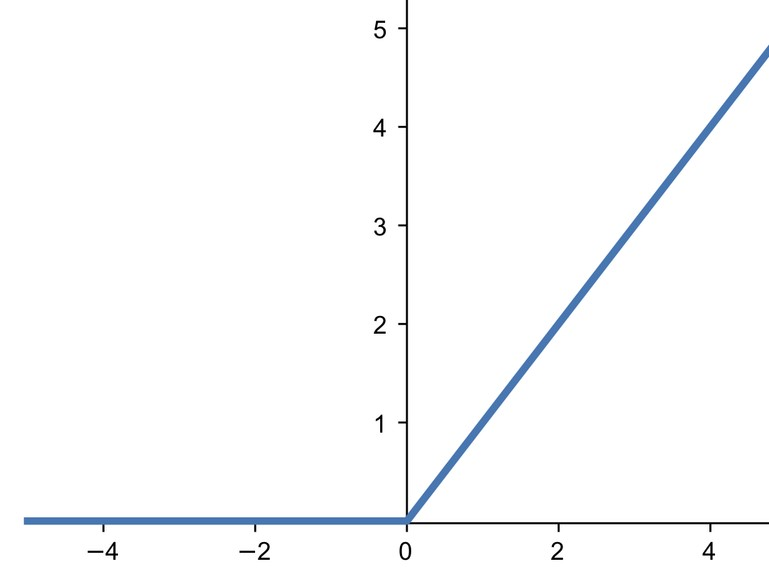
\includegraphics[height=6cm]{../../docs/relu.png}}

\item Sigmoid is another widely used function, it maps every values between 0 and 1. It is defined as $ Sigmoid(z) = \frac{1} {1 + e^{-z}}$ \\
\centerline{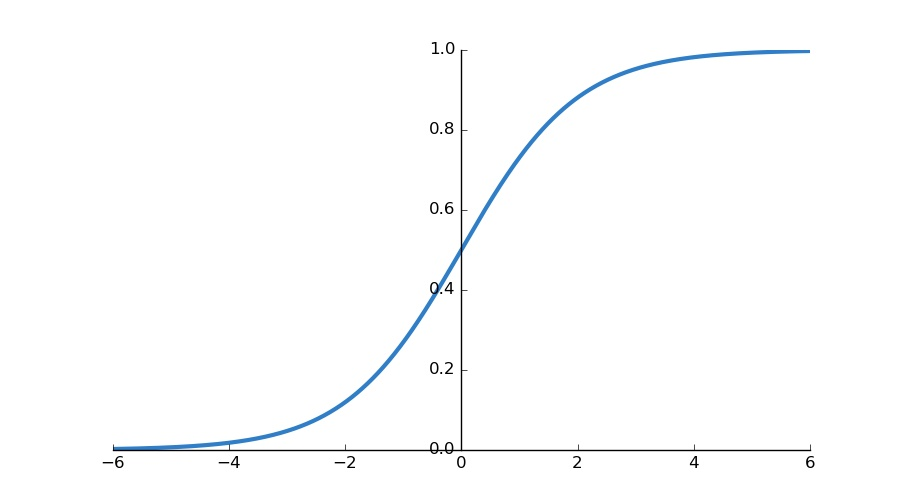
\includegraphics[height=6cm]{../../docs/sigmoid.png}}

\item Tanh, similarly to Sigmoid maps every values between -1 and 1. It is defined as $ Tanh(z) = \frac{1 - e^{-2z}}{1 + e^{-2z}}$ \\
\centerline{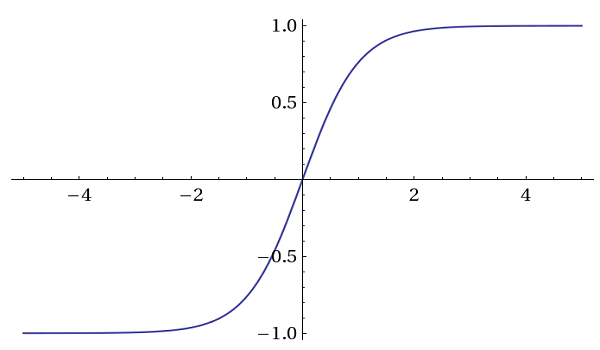
\includegraphics[height=6cm]{../../docs/tanh.png}}

\newpage

\item Softmax is mainly used for single label classification problems. It is defined as $ Softmax(z_i) = \frac{e^{z_{i}}}{\sum_{j=1}^K e^{z_{j}}} \ \ \ for\ i=1,2,\dots,K$ \\
Here is the plot corresponding to the softmax activation for 2 outputs. \\
\centerline{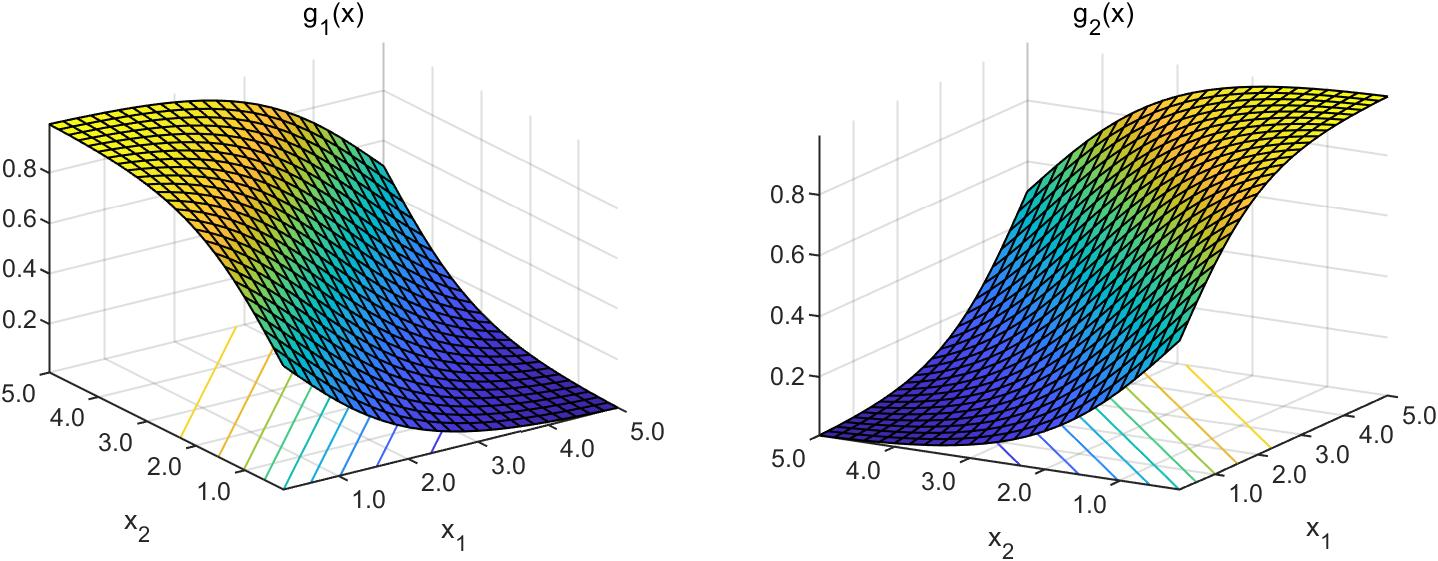
\includegraphics[height=6cm]{../../docs/softmax.png}}

\end{itemize}

% Everyone
\subsection{Model architectures}

So to summarize a bit what was said, a Convolutional Neural Network is a black box that have at least an image as an input and tries to predict something out of this image. As a common trend, the more convolution layers we have, the better our understanding of the image will be. But we have to be careful of how much we should put because we have to keep in mind the performance aspect of our model. In this section, you will see how every member of the team designed their model. \\

\subsubsection{Maxime Gay}
In order to create my model, I was inspired by the VGG-16 model.

This model was proposed by Karen Simonyan and Andrew Zisserman of the Visual Geometry Group Lab of Oxford University in 2014. It won the ImageNet Large Scale Visual Recognition Challenge (ILSVRC) the same year. The model achieves 92.7\% accuracy in ImageNet. By the way, ImageNet is a gigantic database of more than 14 million of images. At this time, it was a sharp evolution regarding the other models because VGG-16 uses kernels of a smaller size.


Architecture of VGG-16 model :

\centerline{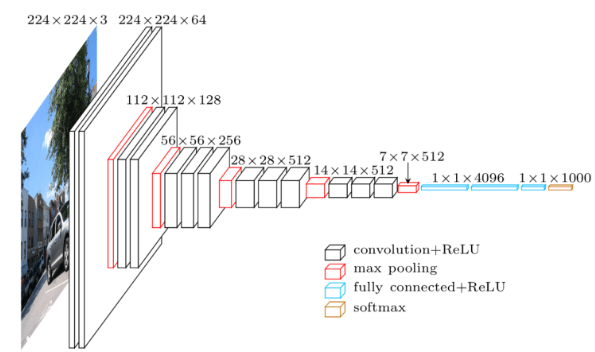
\includegraphics[height=8cm]{../../docs/VGG16.png}}


The VGG-16 architecture is composed of 13 convolutional layers with a 3x3 Kernel separated in five groups.

Between each group there is a pooling layer with a 2x2 size to reduce the size of the filter during the learning phase. At the end of those convolution and pooling layers, there are three Fully-Connected layers and an activation function softmax to determine the class of the image.


The problem of this model is that it is really slow, and it is even slower in our case because it has to work with our car which does not have a lot of resources. Therefore, I decided to change the VGG-16 Model a bit. 
I started by removing some convolutional layers.

My first convolutional layer has a kernel of 5x5 and not 3x3 to have a filter with a bigger size at the beginning. Furthermore, I start with only four kernels on this first layer to reduce the cost of energy.

Then with the others layers, I increased progressively the number of kernels and I reduced the kernel size to 3x3. Moreover, I apply a stride of 2 for the first four layers and a stride of 1 for the last two. At the end, I use two Dense layers with an activation function "relu" like the others layers.


Furthermore, I tested many different optimizer like SGC, Adadelta, Nadam and Ftrl but I decided to use the Adam Optimizer because it gave me the best result. The Adam optimizer involves a combination of two gradient descent methodologies.


\subsubsection{Mickael Bobovitch}
\subsubsection{Alexandre Girold}
For my part, I decided to 

\subsubsection{Maxime Ellerbach}
When I started to make my model, I thought about: "What could make my model different from the others ?" When looking at what my teammates did, it is obvious that the main difference in the model is not in the architecture itself of the model but rather in the data that is fed to it. One other observation is that the less parameters we have in the model, the less sensible it is to overfitting, so the main idea was to have a light model that would also have a rather small latent space. \\

I did see that the combination of [Layer $\rightarrow$ Relu Activation $\rightarrow$ BatchNormalization] worked better with unseen testing images, so I did use this combination for every convolution and Dense layers. \\



\begin{figure}[h]
    \centering
    \subfloat[Model MaximeE]{%
        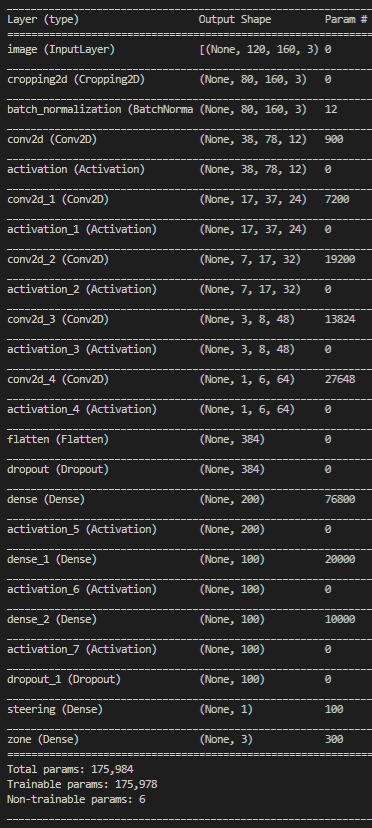
\includegraphics[height=0.49\textheight]{../../docs/model-maxe.png}%
        \label{fig:a}%
        }%
    \subfloat[Model MaximeG]{%
        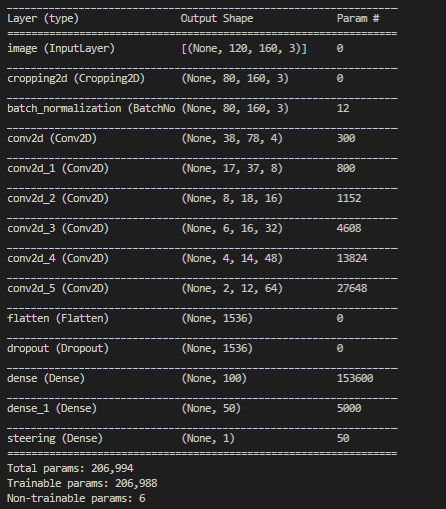
\includegraphics[height=0.49\textheight]{../../docs/model-maxg.png}%
        \label{fig:b}%
        }%
    \hfill %
    \subfloat[Model AlexandreG]{%
        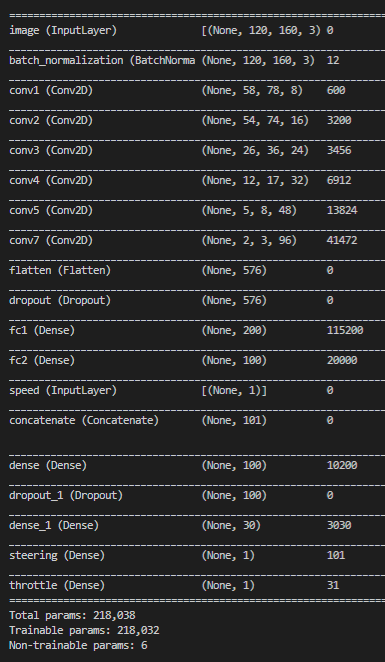
\includegraphics[height=0.49\textheight]{../../docs/model-sacha.png}%
        \label{fig:b}%
        }%
    \subfloat[Model MickaelB]{%
        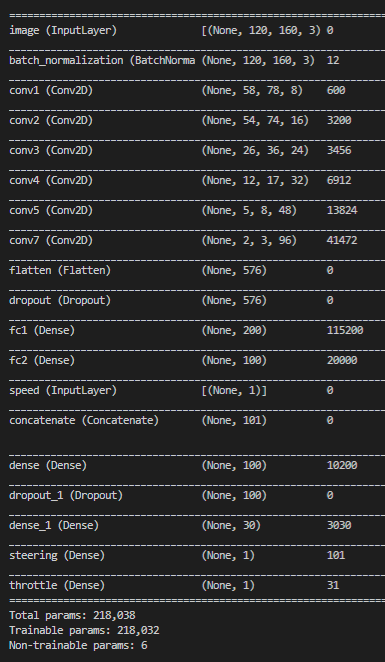
\includegraphics[height=0.49\textheight]{../../docs/model-sacha.png}%
        \label{fig:a}%
        }%
    \caption{Model Architectures}
\end{figure}


% Girold & Gay
\subsection{Load data during training}

% Girold
\subsection{Training Process}

After loading our data, we need to be able to train on those loaded data. The training process is where everything takes place. Indeed, training the data requires the use of all the previous functions. One of these functions is the settings.py. You can see how the function works with the small example below.

\centerline{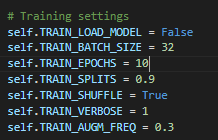
\includegraphics[height=4cm]{../../docs/setting-train.png}}

This function is the backbone of the training process. It allows us to have a very modular project where everything can be modified from this file only. This allow us to modify our project without deleting a lot of code, making it very modular which was one of our goals from the beginning. For example, we have recently added the telemetry server's restart function, once it was created, we only had to add it to the settings.py and all the other functions would be able to use it.   
This is also useful to change values in real-time. For example, if we want to train our model on more epochs or that our computer can handle bigger batch sizes then we only must change one value and that is it. This goes for all the functions in our project. 

The second import function is of course the train.py function.

At first, this function creates all our useful variables (imported from the settings).  Then if the given model doesn’t exist, we create it, for now, this model hasn’t yet been trained.  Then we need to feed the make sure all the variables are correct so the model can be trained.  To train a model we need data, in our case images. For this we need to make sure those data exist, and that the path to them is correct.  
We also want to know all the inputs and outputs. This is important as we might want to train not only the steering but also the throttle and speed.  
Finally, we use one important training library. The .fit library from karas. With fit, we are first feeding the training data(X) and training labels(Y) in our case these X and Y come from DataGenerator. We then use Keras to allow our model to train for a given number of epochs and on a given amount of batch sizes. 

% Bobovitch
\subsection{Data Augmentation}



\newpage

% sout : 7 / 03 & 25 / 04 & 06 / 06
\section {Planning}
\subsubsection {What is next ?}
The objectives we set ourselves for this presentation were acheived, for the next intermediate presentation we plan to finish what we are currently working on meaning The telemetry server and the logging. Moreover, we also plan to have a working prototype of the whole car including the AI part with the development of a basic convolutional neural network in a first time. This means we will have to create a model, then have a script to train it using collected data and finally a script to drive our car using this trained model.

\subsubsection {Races}

\begin{tabular}{|l|c|c|c|c|c|c|}
\hline
Tasks & Race 1 & Race 2 & Race 3 & Race 4 & Race 5 & Race 6  \\ 
\hline
Code controlled motors and servo                & 75\%   & 100\%  &        &        &        &         \\ 
\hline
Drive the car with a controller                 & 25\%   & 100\%   &        &        &        &         \\ 
\hline
Data collection                                 &        & 50\%   & 100\%  &        &        &         \\ 
\hline
Telemetry server                                &        & 25\%   & 100\%  &        &        &         \\ 
\hline
Logging                                         &        & 25\%   & 100\%  &        &        &         \\ 
\hline
Data processing and augmentation                &        &        & 50\%   & 75\%   & 100\%  &         \\ 
\hline
Basic Convolutional neural network              &        &        & 25\%   & 50\%   & 100\%  &         \\ 
\hline
\begin{tabular}[c]{@{}l@{}}Advanced \\models and optional objectives\end{tabular} &        &        &        &        &        & 50\%    \\
\hline
\end{tabular}

\subsection {Presentations}

\begin{tabular}{|l|c|c|c|} 
\hline
Tasks                                                                             & 1st presentation & 2nd Presentation & Final presentation  \\ 
\hline
Code controlled motors and servo                                                  & 100\%              &                &                    \\ 
\hline
Drive the car with a controller                                                   & 100\%              &                &                    \\ 
\hline
Data collection                                                                   & 75\%               & 100\%          &                    \\ 
\hline
Telemetry server                                                                  & 25\%               & 100\%          &                    \\ 
\hline
Logging                                                                           & 25\%               & 100\%          &                    \\ 
\hline
Presentation website                                                              & 100\%              & Update         & Update             \\ 
\hline
Data processing and augmentation                                                  &                    & 75\%           & 100\%              \\ 
\hline
Basic Convolutional neural network                                                &                    & 50\%           & 100\%              \\ 
\hline
\begin{tabular}[c]{@{}l@{}}Advanced \\models and optional objectives\end{tabular} &                    &                & 50\%               \\
\hline
\end{tabular}


\section {Task allocation}

\begin{tabular}{|l|c|c|c|c|} 
\hline
Tasks                        & Mickael B. & Maxime G. & Alexandre G. & Maxime E.  \\ 
\hline
Low level car control        &            &           &              & x          \\ 
\hline
Driving with a controller    &            & x         & x            & x          \\ 
\hline
Dataset handling             &            & x         & x            &            \\ 
\hline
Data processing              & x          & x         & x            & x          \\ 
\hline
Data visualization           &            &           &              & x          \\ 
\hline
Telemetry server             & x          &           &              & x          \\ 
\hline
Logging                      & x          &           &              & x          \\ 
\hline
Presentation website         & x          &           &              &            \\ 
\hline
Convolutional neural network & x          & x         & x            & x          \\ 
\hline
Main control loop            & x          &           &              &            \\
\hline
\end{tabular}

\section {Conclusion}
To sum up, Autonomobile team improved the control of the car with controller, furthermore the data processing is working flawlessly allowing us to load and save images and metadata. Moreover, our presentation website is ready, it includes the presentation of the team, some links to download our project and even a road map. Nevertheless, the hardest part is yet to come, indeed we have to work on the AI part of the car and on the telemetry website to have it working by the next project defense.\\
The telemetry website is important in order to visualize data to know what is happening inside the car at any moment. We will have to work and learn a lot on this topic which is fascinating.\\

To make a long story short, we spent a lot of time on this project, which comport many sections that are important for the realization of this project, and we will do every thing to succeed. 


\end{document}
